

\clearpage
\subsection{Digital Signal Post-Processing}
The stages of the DSP process applied to the experimental results of this setup are presented in Figure~\ref{fig:mqamDiagramDSP}. 	
%
\begin{figure}[h]
\centering
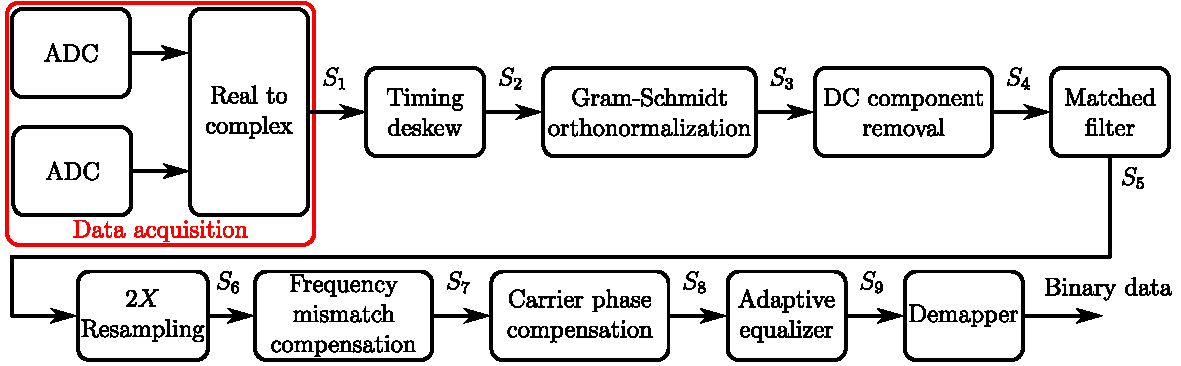
\includegraphics[width=\linewidth]{./sdf/m_qam_system/figures/DSP_section/diagramDSP}
\caption{Block diagram of the DSP applied offline in the netxpto environment.}
\label{fig:mqamDiagramDSP}
\end{figure}
%
After conversion to digital and combination in a complex vector, the signal is first passed through a timing-deskew process, in which IN PROGRESS
\par
%
The constellation on which the DSP will be implemented is presented in Figure~\ref{fig:inConstellation_DSP}. This data was obtained from the .mat file  \textbf{SNR=38\_trial8\_.mat}, included in the folder \textit{$\backslash$sdf$\backslash$m\_qam\_system\_dsp$\backslash$Data}. A short matlab code present in same folder, named \textbf{mat2txt.m}, reads the \textbf{.mat} file and outputs the received signal to a text file named \textbf{Input.txt}. This \textbf{.txt} file can be read into the netxpto environment by using the \textit{LoadAscii} block, the code necessary for this is included below.
\begin{verbatim}
TimeContinuousAmplitudeContinuousComplex SIn{ "SIn.sgn" };

LoadAscii BI{ {}, { &SIn } };
BI.setAsciiFileName("Input.txt");
BI.setDataType(ComplexValue);
BI.setDelimiterType(delimiter_type::CommaSeperatedValues);
BI.setSamplingPeriod(1 / 50e9);
BI.setSymbolPeriod(1 / 1.25e9);
\end{verbatim}
After loading the signal to the netxpto environment for a first time, it is saved in the \textbf{.sgn} format, this version of the signal can then be loaded into the netxpto environment with the \textit{LoadSignal} block, the code necessary for this is included below.
\begin{verbatim}
TimeContinuousAmplitudeContinuousComplex S1{ "S1.sgn" };

LoadSignal BI{ {}, { &S1 } };
BI.setSgnFileName("SIn.sgn");
\end{verbatim}

This constellation was obtained by downsampling the signal obtained from the oscilloscope down to 1 sample per symbol and roughly centering the sampling point to its peaks.
%
\begin{figure}[h]
\centering
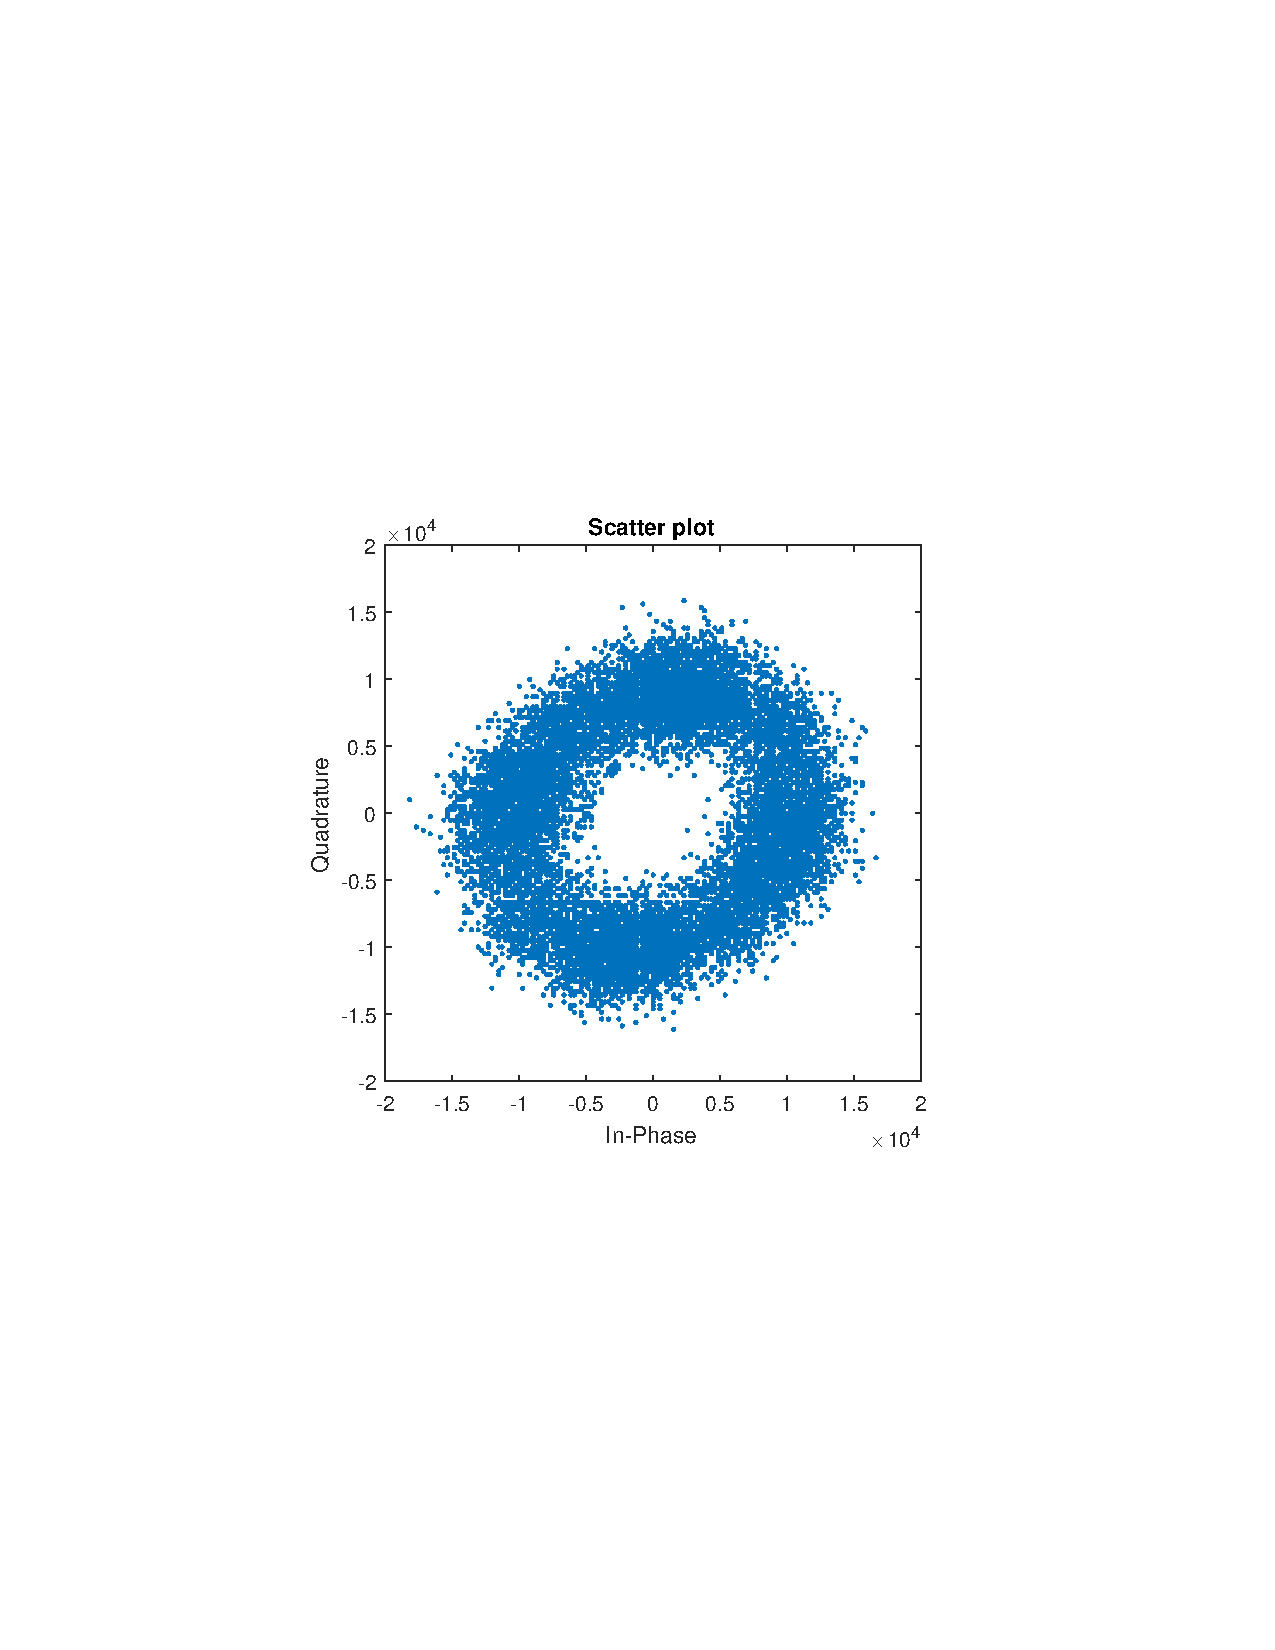
\includegraphics[trim={7cm 8cm 7cm 8cm},width=.4\linewidth]{./sdf/m_qam_system/figures/DSP_section/initialConstellation}
\caption{Constellation obtained at the oscilloscope from a signal with a baud rate of 1.25~Gbd and a SNR of 38~dB.}
\label{fig:inConstellation_DSP}
\end{figure}	
%
All DSP steps applied to this constellation are now described one by one.

\subsubsection{Timing deskew}

This DSP step takes a complex input signal and removes a given amount of timing skew between its real (in-phase) and imaginary (quadrature) parts. This DSP step follows the topology presented in Figure~\ref{fig:mqamDiagramDSP_DS}
%
\begin{figure}[h]
\centering
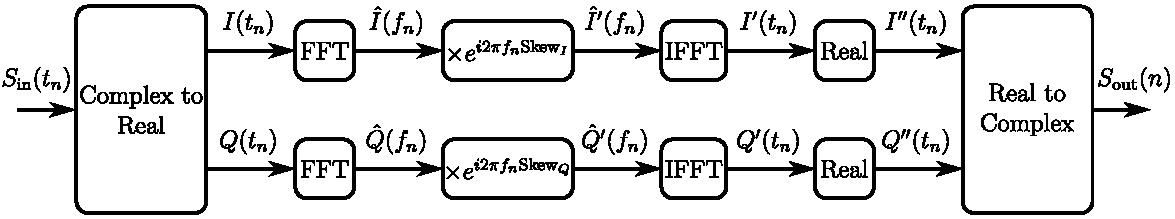
\includegraphics[width=\linewidth]{./sdf/m_qam_system/figures/DSP_section/diagramDSP_DS}
\caption{Block diagram representation of the deskew procedure.}
\label{fig:mqamDiagramDSP_DS}
\end{figure}
%
The input signal $S_\text{in}(n)$ is separated into its in-phase and in-quadrature components, $I(n)$ and $Q(n)$, both components are transformed to Fourier space, where they are multiplied by a deskew element
%
\begin{align}
\hat{I}^\prime(f_n)&=\hat{I}(f_n) e^{i2\pi f_n \text{Skew}_I},\\
\hat{Q}^\prime(f_n)&=\hat{Q}(f_n) e^{i2\pi f_n \text{Skew}_Q}.
\end{align}
%
These two components are then transformed back to time domain, the imaginary part of each component is discarded and the resulting components are combined to form the output signal

\begin{equation}
S_\text{out}(t_n)=\text{real}(I^\prime(t_n))+i\text{real}(Q^\prime(t_n)).
\end{equation}
\par
The effect of this DSP step is presented in Figure~\ref{fig:S2}.
%
\begin{figure}[h]
\centering
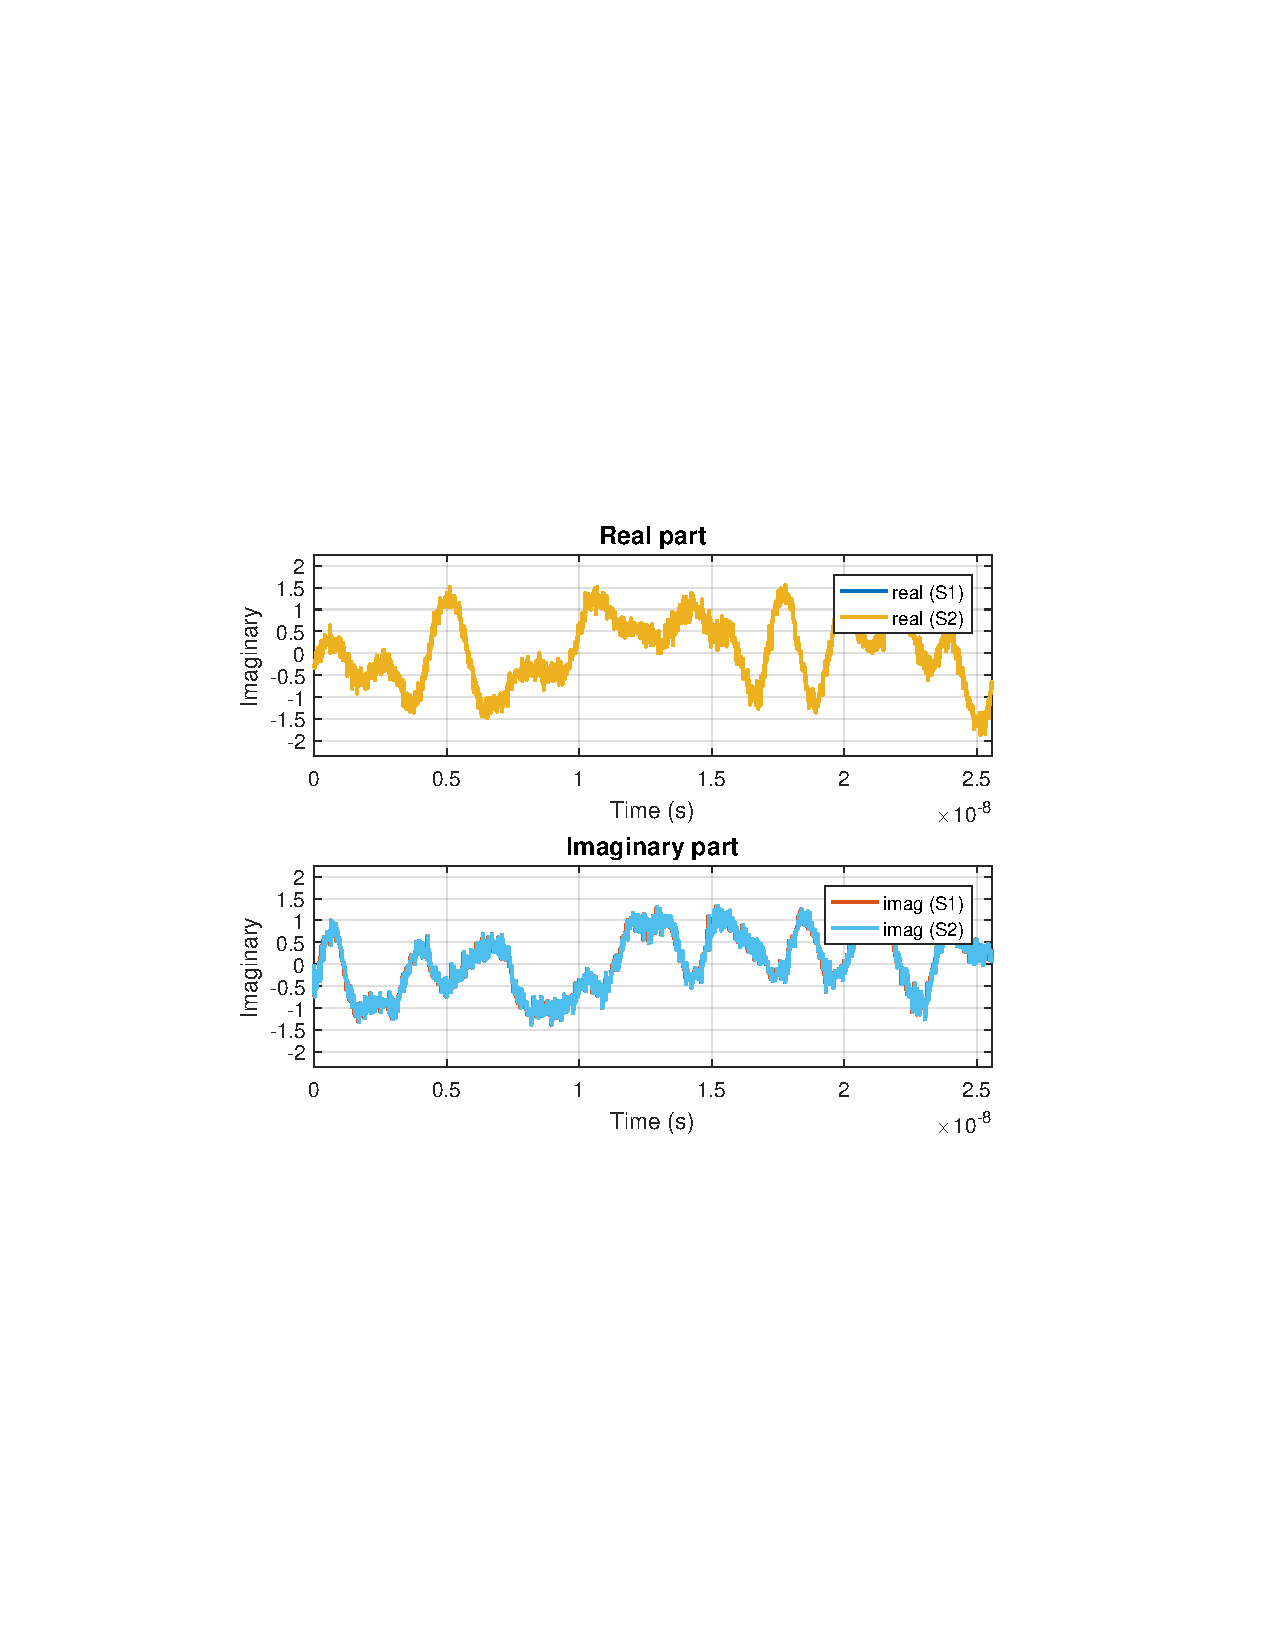
\includegraphics[trim={7cm 8cm 7cm 8cm},width=.3\linewidth]{./sdf/m_qam_system/figures/DSP_section/S2}
\caption{Signals before and after deskew DSP step.}
\label{fig:S2}
\end{figure}	
%

\subsubsection{Gram-Schmidt orthonormalization}

This step orthonormalizes the data by implementing a Gram-Schmidt algorithm. This is implementation follows the topology presented in Figure~\ref{fig:mqamDiagramDSP_GS}.
%
\begin{figure}[h]
\centering
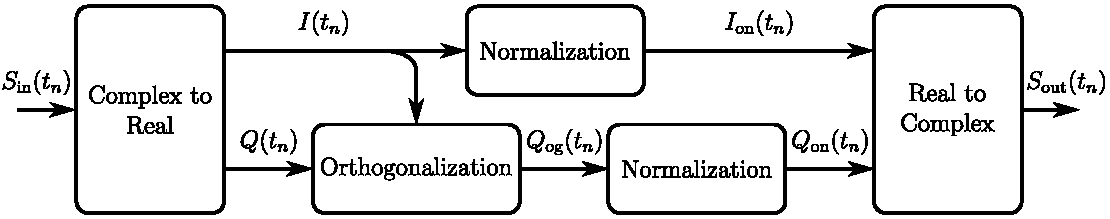
\includegraphics[width=\linewidth]{./sdf/m_qam_system/figures/DSP_section/diagramDSP_GS}
\caption{Block diagram representation of the Gram-Schmidt orthonormalization procedure.}
\label{fig:mqamDiagramDSP_GS}
\end{figure}
%
The input signal $S_\text{in}(t_n)$ is separated into its in-phase and in-quadrature components, $I(t_n)$ and $Q(t_n)$, the amplitude of the in-phase component, $P_I$, is estimated as the average of its square, ie.:
\begin{equation}
P_I=\text{mean}(I^2(t_n)),
\end{equation}
the in-phase signal is then normalized, ie.:
\begin{equation}
I_\text{on}(t_n)=\frac{I(t_n)}{\sqrt{P_I}}.
\end{equation}
The in-quadrature component is then orthogonalized in relation to the in-phase component
\begin{equation}
Q_\text{og}(t_n)=Q(t_n)-\frac{I(t_n)\text{mean}(I(t_n)Q(t_n))}{P_I},
\end{equation}
which is then normalized in a manner similar to what was done for the in-phase component
\begin{align}
P_Q=\text{mean}(Q_\text{og}^2(t_n)),\\
Q_\text{on}(t_n)=\frac{Q_\text{og}(t_n)}{\sqrt{P_Q}}.
\end{align}
Finally, the two orthonormalized components are combined to form the output signal
\begin{equation}
S_\text{out}(t_n)=I_\text{on}(t_n)+iQ_\text{on}(t_n)
\end{equation}
%\par
The effect of this DSP step is presented in Figure~\ref{fig:S3II}.
\begin{figure}[h]
\centering
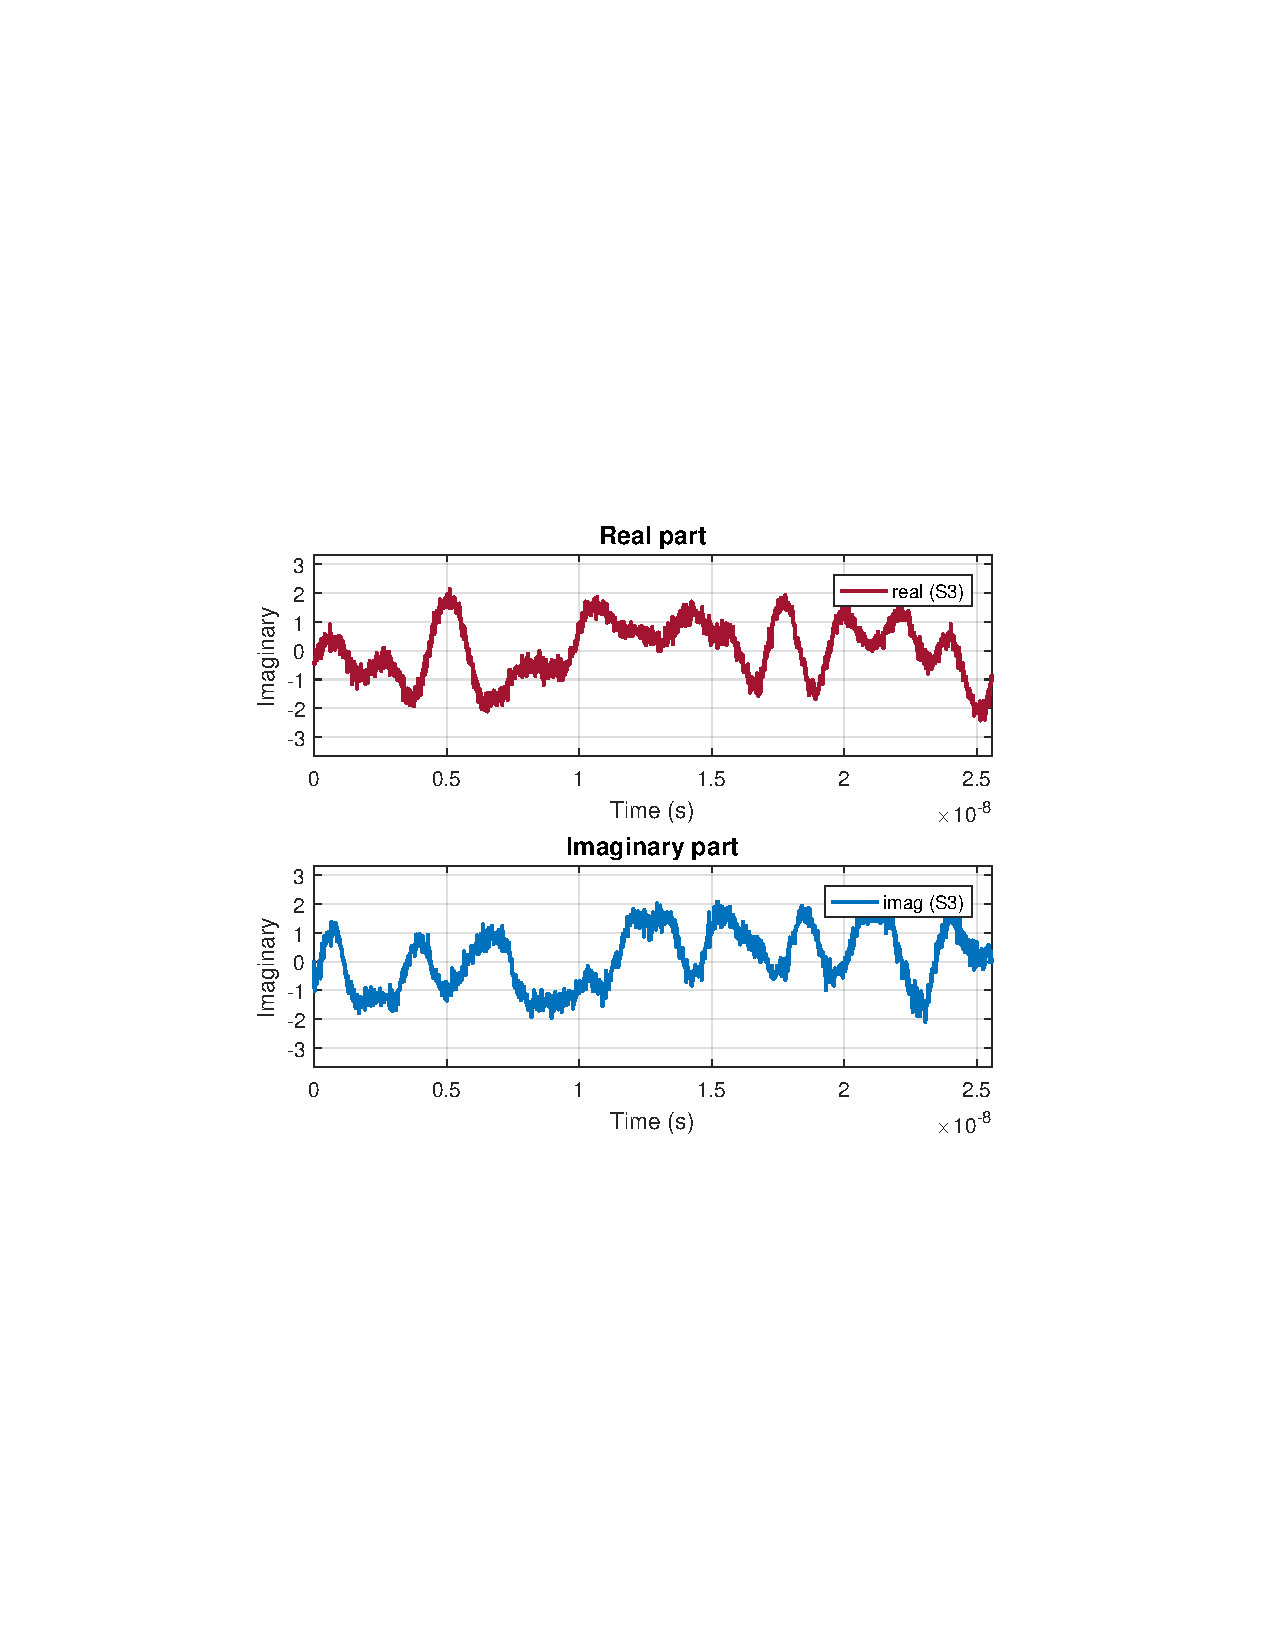
\includegraphics[trim={7cm 8cm 7cm 8cm},width=.3\linewidth]{./sdf/m_qam_system/figures/DSP_section/S3II}
\caption{Signal after orthonormalization DSP step.}
\label{fig:S3II}
\end{figure}	
%
\subsubsection{DC component removal}

This DSP step removes the DC contribution on the input signal ,$S_\text{in}(t_n)$. This DC contribution can either be estimated by taking the average of the full input signal or from the average of a moving window. This contribution is then subtracted from the input
\begin{equation}
S_\text{out}(t_n)=S_\text{in}(t_n)-\text{mean}(S_\text{in}(t_n))
\end{equation}
\par
The effect of this DSP step is presented in Figure~\ref{fig:S4}.
%
\begin{figure}[h]
\centering
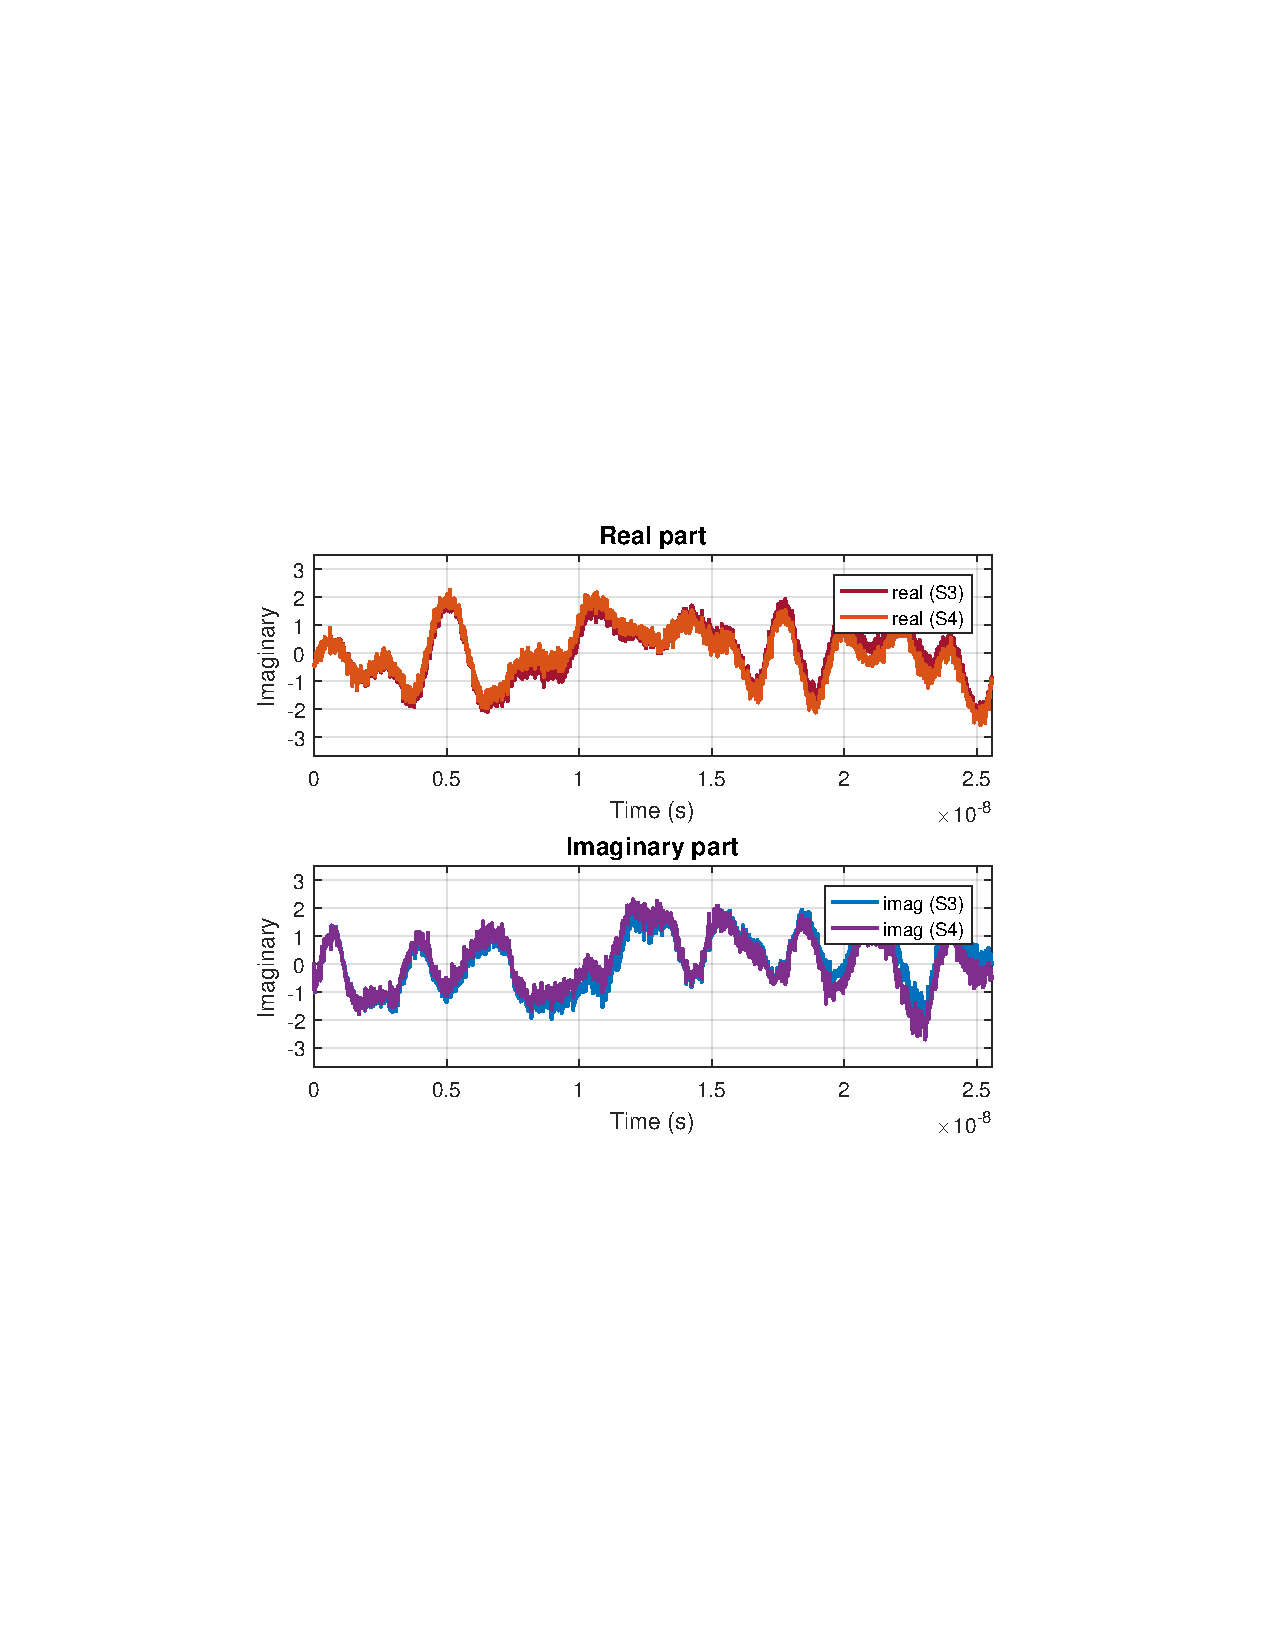
\includegraphics[trim={7cm 8cm 7cm 8cm},width=.3\linewidth]{./sdf/m_qam_system/figures/DSP_section/S4}
\caption{Signals before and after DC component removal DSP step.}
\label{fig:S4}
\end{figure}	
%

\subsubsection{Matched filtering}

This step implements some form of matched filtering. For the modulation of the signal corresponding to the constellation in Figure~\ref{fig:inConstellation_DSP}, the matched filter consists of a root raised cosine function. The filter can be applied either in time-domain, through convolution of the signal with the filtering function, or in frequency domain, through a simple multiplication.
\par
The effect of this DSP step is presented in Figure~\ref{fig:S5}.
%
\begin{figure}[h]
\centering
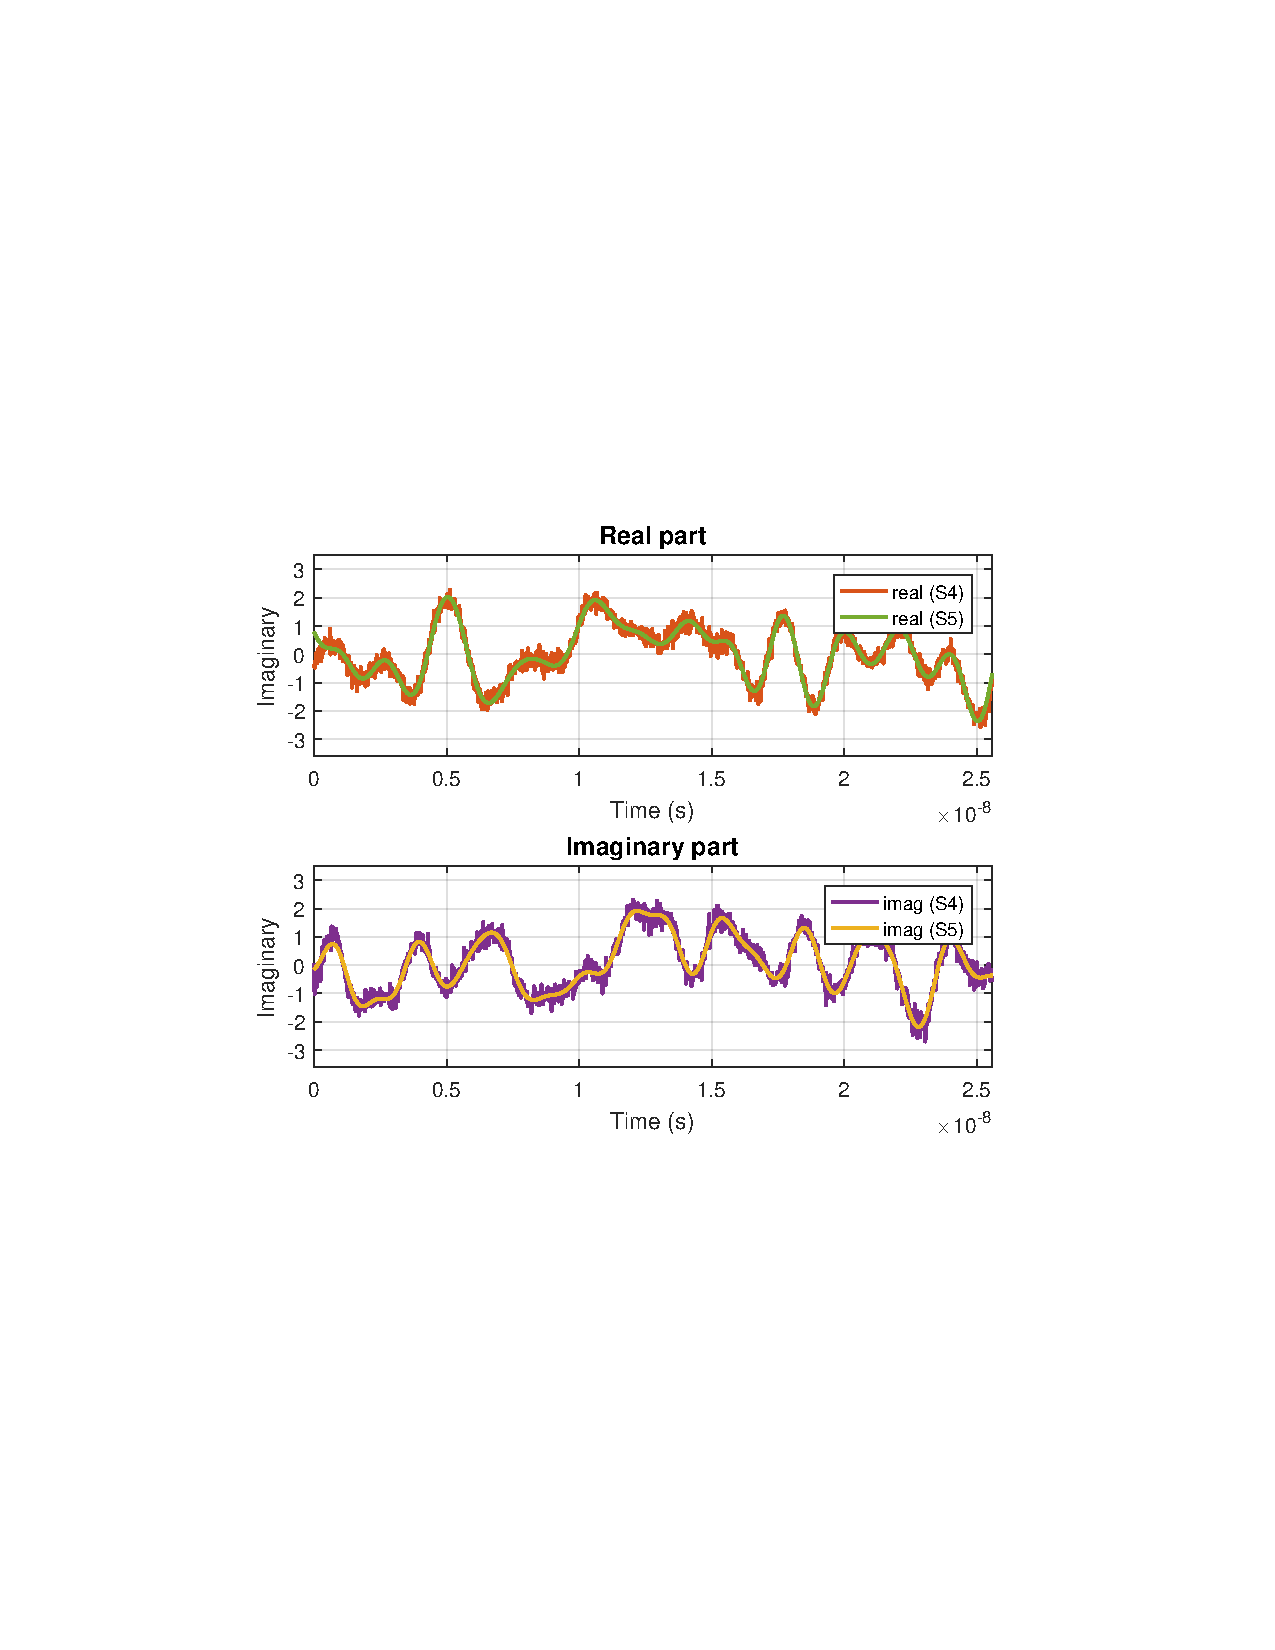
\includegraphics[trim={7cm 8cm 7cm 8cm},width=.3\linewidth]{./sdf/m_qam_system/figures/DSP_section/S5}
\caption{Signals before and after matched filtering.}
\label{fig:S5}
\end{figure}	
%

\subsubsection{2$\times$ resampling}

This step consists of a digital resampling that effectively doubles the sampling rate of the signal, with the values of the new points filled using a polyphase anti-aliasing filter.

\subsubsection{Frequency mismatch compensation}

This step compensates for the frequency mismatch between the local oscillators employed at the transmission and reception stages. Multiple methods for this are available, the one employed for the results presented here is the spectral method, a topological representation of which is presented in Figure~\ref{fig:mqamDiagramDSP_FE_spectral}.
%
\begin{figure}[h]
\centering
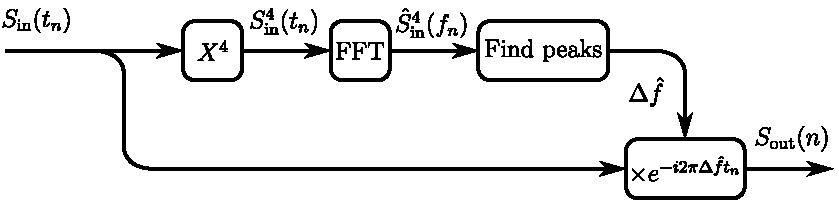
\includegraphics[width=.7\linewidth]{./sdf/m_qam_system/figures/DSP_section/diagramDSP_FE_spectral}
\caption{Block diagram representation of the spectral frequency mismatch estimation and compensation procedure.}
\label{fig:mqamDiagramDSP_FE_spectral}
\end{figure}
%
The input signal, which can be described as
\begin{equation}
S_\text{in}(t_n)=|S_\text{in}(t_n)|e^{i\left(2\pi\Delta f t_n+\theta(t_n)+\Delta\phi\right)},
\end{equation}
is powered by 4, yielding
\begin{equation}
S^4_\text{in}(t_n)=|S_\text{in}(t_n)|e^{i\left(2\pi4\Delta f t_n+4\theta(t_n)+4\Delta\phi\right)},
\end{equation}
since $\theta(t_n)\in\left\lbrace \frac{\pi}{4},\frac{3\pi}{4},\frac{5\pi}{4},\frac{7\pi}{4}\right\rbrace$, we get
\begin{equation}
S^4_\text{in}(t_n)=|S_\text{in}(t_n)|e^{i\left(2\pi4\Delta f t_n+\pi+4\Delta\phi\right)},
\end{equation}
so this process effectively removes the QPSK modulation of the signal. The $S^4_\text{in}(t_n)$ signal is then converted to the frequency domain, because of the removal of the phase modulation, its spectrum is expected to display a maximum at a frequency of $4\Delta f$, which is determined by some \textit{find peaks} function, yielding the estimate $\Delta\hat{f}$. The input signal $S_\text{in}$ is then multiplied by $e^{-i2\pi\Delta\hat{f}t_n}$. Assuming the estimate is a good one, this process will remove the effect of the frequency mismatch, yielding the following output signal
\begin{equation}
S_\text{out}(t_n)=S_\text{in}(t_n)e^{-i2\pi\Delta\hat{f}t_n}=|S_\text{in}(t_n)|e^{i\left(\theta(t_n)+\Delta\phi\right)}
\end{equation}

\subsubsection{Carrier phase compensation}

This step compensates for the phase mismatch between the local oscillators employed at the transmission and reception stages. Multiple methods for this are available, the one employed for the results presented here is the blind method, a topological representation of which is presented in Figure~\ref{fig:mqamDiagramDSP_CPE_blind}.
%
\begin{figure}[h]
\centering
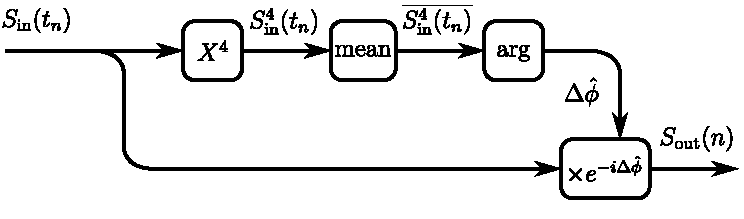
\includegraphics[width=.7\linewidth]{./sdf/m_qam_system/figures/DSP_section/diagramDSP_CPE_blind}
\caption{Block diagram representation of the blind phase mismatch estimation and compensation procedure.}
\label{fig:mqamDiagramDSP_CPE_blind}
\end{figure}
%
The input signal, which at this stage can be described as
\begin{equation}
S_\text{in}(t_n)=|S_\text{in}(t_n)|e^{i\left(\theta(t_n)+\Delta\phi\right)},
\end{equation}
is powered by 4, yielding
\begin{equation}
S^4_\text{in}(t_n)=|S_\text{in}(t_n)|e^{i\left(4\theta(t_n)+4\Delta\phi(t_n)\right)},
\end{equation}
since $\theta(t_n)\in\left\lbrace \frac{\pi}{4},\frac{3\pi}{4},\frac{5\pi}{4},\frac{7\pi}{4}\right\rbrace$, we get
\begin{equation}
S^4_\text{in}(t_n)=|S_\text{in}(t_n)|e^{i\left(\pi+4\Delta\phi(t_n)\right)},
\end{equation}
so this process effectively removes the QPSK modulation of the signal. The average of the $S^4_\text{in}(t_n)$ signal is then computed and its phase evaluated, yielding the estimate $4\Delta \hat{\phi}$. The input signal $S_\text{in}$ is then multiplied by $e^{-i\Delta\hat{\phi}}$. Assuming the estimate is a good one, this process will remove the effect of the phase mismatch, yielding the following output signal
\begin{equation}
S_\text{out}(t_n)=S_\text{in}(t_n)e^{-i\Delta\hat{\phi}}=|S_\text{in}(t_n)|e^{i\theta(t_n)}
\end{equation}

\subsubsection{Adaptive equalizer}
